
\chapter{Introduction to SPAMDA}

	\begin{onehalfspace}

		\section{SPAMDA description}

			SPAMDA is a software tool for creating datasets with meteorological data from two well-known sources of information, \textit{National Data Buoy Center} (NDBC) \cite{NOAA} and \textit{Reanalysis Project} (NNRP or R1) \cite{Kalnay1996, Kistler2001}.
			
			The datasets created with SPAMDA will be ready to use as input for Machine Learning (ML) techniques in classification or regression prediction tasks, although the researchers may use them in the way they deem suitable. These datasets will contain one or more meteorological variables as inputs and another one as target (variable to predict). The format of the datasets will be \textit{Attribute-Relation File Format} (ARFF) \cite{WEKA_ARFF} that it is used by the well-known tool \textit{Waikato Environment for Knowledge Analysis} (WEKA) \cite{WEKA}, which provides a wide collection of ML algorithms. Besides, the datasets can also be generated in \textit{Comma-Separated Values} (CSV) format, enabling the researchers to use others tools.
			
			Some of the advantages that SPAMDA tool offers are briefly summarised below:

				\begin{itemize}
					\item The generation of datasets becomes a very easy and customizable task, by means of the selection of different input parameters.
					\item It makes the researcher focus on oceanic and atmospheric studies, without having to worry about mechanical tasks.
					\item It provides information about the quality and quantity of the data.
					\item It avoids possible researcher errors in the intermediate steps of the process of creation of the datasets.
					\item It includes different pre-processing tasks, such as normalisation and missing data recovery.
					\item It facilitates data management and well-organised storage of the datasets.
					\item Its modular design allows the implementation of new functional modules for managing meteorological data from others sources for renewable energy research.
					\item It includes an user-friendly GUI, facilitating and greatly simplifying data management, and it is integrated with the Explorer environment of WEKA.
					\item It is multi-platform, and it can be used on any computer with Java regardless of the operating system.
				\end{itemize}
				
	\section{Meteorological data sources}\label{sec:DataSources}
		
		The data provided by the above-mentioned sources of information used by SPAMDA is briefly described below:
		
		\begin{itemize}

			\item NDBC is a part of the \textit{National Weather Service} (NWS). NDBC designs, develops, operates, and maintains a network of data collecting buoys (stations). The mission of the network is to collect real-time marine meteorological and oceanographic observations, such as wave height, dominant wave period, or wind speed and direction, among others.

			The buoys maintained by NDBC are deployed in the coastal and offshore waters around oceans and seas, and are equipped with assorted sensors which allow them to perform different measurements. The information collected by the buoys is available in NDBC web page \cite{NOAA_1}, which is divided into different groups. One of them is the standard meteorological information of the historical data collected by each buoy, which can be downloaded as annual text files and whose format was adopted by NDBC since January 2007 \cite {NOAA_2}. These files contain hourly measurements per day from $00$:$50$ to $23$:$50$ UTC and from $23$:$50$ 31th Dec of the previous desired year to $22$:$50$ 31th Dec of the desired year. In Table \ref{tab:measurementsDescription} a comprehensive measurements descriptions and units of such information is provided.
			
			\clearpage
			
			\begin{table}[ht!]
			
				\caption{Measurements descriptions and units of each meteorological variable or attribute collected by the buoys.}
				\label{tab:measurementsDescription}
				\footnotesize
				\centering
				
				\begin{tabular}{ccm{11.00cm}@{\setlength{\tabcolsep}{0pt}}m{0.0cm}}
				
					\cline{1-4}
					
					%\textbf{Variable}&\textbf{Units}&\textbf{Description}&\\[0.30cm]
					
					\textbf{Attribute}&\textbf{Units}&\textbf{Description}&\\[0.30cm]
 
					\cline{1-4}
					
					WDIR & degT & Wind direction (the direction the wind is coming from in degrees clockwise from true N) during the same period used for WSPD. \\
					
					\cellcolor{gray090}WSPD & \cellcolor{gray090} m/s & \cellcolor{gray090} Wind speed (m/s) averaged over an eight-minute period for buoys and a two-minute period for land stations. Reported Hourly. \\
					
					GST &  m/s & Peak 5 or 8 second gust speed (m/s) measured during the eight-minute or two-minute period. \\
					
					\cellcolor{gray090} WVHT & \cellcolor{gray090} m & \cellcolor{gray090} Significant wave height (meters) is calculated as the average of the highest one-third of all of the wave heights during the 20-minute sampling period. \\
					
					DPD & sec & Dominant wave period (seconds) is the period with the maximum wave energy. \\
					
					\cellcolor{gray090}APD & \cellcolor{gray090} sec & \cellcolor{gray090} Average wave period (seconds) of all waves during the 20-minute period. \\
					
					MWD & degT & The direction from which the waves at the dominant period (DPD) are coming. The units are degrees from true North, increasing clockwise, with North as 0 (zero) degrees and East as 90 degrees. \\
					
					\cellcolor{gray090}PRES & \cellcolor{gray090} hPa & \cellcolor{gray090} Sea level pressure (hPa). For C-MAN sites and Great Lakes buoys, the recorded pressure is reduced to sea level using the method described in NWS Technical Procedures Bulletin 291 (11/14/80). \\
					
					ATMP & degC & Air temperature (Celsius). &\\[0.10cm]
					
					\cellcolor{gray090}WTMP & \cellcolor{gray090} degC & \cellcolor{gray090} Sea surface temperature (Celsius). For buoys the depth is referenced to the hull's waterline. For fixed platforms it varies with tide, but is referenced to, or near Mean Lower Low Water (MLLW).\\
					
					DEWP & degC & Dewpoint temperature taken at the same height as the air temperature measurement. \\
					
					\cellcolor{gray090}VIS & \cellcolor{gray090} nmi & \cellcolor{gray090} Station visibility (nautical miles). Note that buoy stations are limited to reports from 0 to 1.6 nmi. \\
					
					%PTDY & hPa & Pressure Tendency is the direction (plus or minus) and the amount of pressure change (hPa) for a three hour period ending at the time of observation. \\
					
					TIDE & ft & The water level in feet above or below Mean Lower Low Water (MLLW). \\
					
					\cline{1-4}
						
				\end{tabular}
			 
			\end{table}

			
			\item NNRP provides three-dimensional global reanalysis of numerous meteorological variables (e.g. air temperature, U/V-wind, relative humidity, pressure, etc.), which is available monthly, daily and every $6$ hours at $00$Z, $06$Z, $12$Z and $18$Z from $1948$ on a global $2.5\degree$ x $2.5\degree$ grid. Weather observations are from different sources, such as ships, satellites and radar, among others.
			
			%The reanalysis data is available in NNRP web page \cite{NNRP}, which are accessible through the different sections. Such data can be fully (a global $2.5\degree$ x $2.5\degree$ grid) or partially (only the desired reanalysis nodes or sub-grid) downloaded as \textit{Network Common Data Form} (NetCDF) files \cite{NetCDF}, a special binary format for representing scientific data which provides a description of what the data in each variable represents and the spatial and temporal properties of the data. Each reanalysis data file contains the estimated values by a mathematical model of one meteorological variable and for each reanalysis node. For a better understanding, in Fig. \ref{fig:subGrid} an approximate representation of a six sub-grid reanalysis nodes around the geographical localisation of a buoy (obtained from NDBC) is shown.
			
			The reanalysis data is available in NNRP web page \cite{NNRP}, which are accessible through the different sections. Such data can be fully (a global $2.5\degree$ x $2.5\degree$ grid) or partially (only the desired reanalysis nodes or sub-grid) downloaded as \textit{Network Common Data Form} (NetCDF) files \cite{NetCDF}, a special binary format for representing scientific data which provides a description of the file contents and also includes the spatial and temporal properties of the data. Each reanalysis file contains the values of a meteorological variable estimated by a mathematical model for each reanalysis node. For a better understanding, in Fig. \ref{fig:subGrid} an approximate representation of a sub-grid containing six reanalysis nodes around the geographical localisation of a buoy (obtained from NDBC) is shown.
			
			\begin{figure}[ht!]
				\centering
				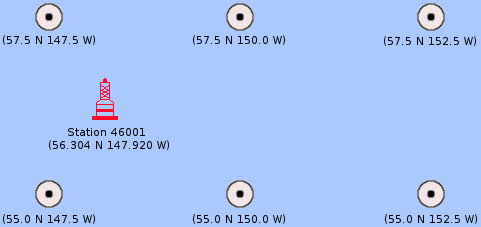
\includegraphics[scale=0.52]{figures/FigureSubGrid.jpg}
				\caption{Example of a six sub-grid reanalysis nodes around the \textit{Station 46001}.}
				\label{fig:subGrid}
			\end{figure}
			
		\end{itemize}
		
		With both sources of information SPAMDA will create datasets for prediction tasks. In this way, the input variables of the dataset will be one or more reanalysis variables from NNRP and one or more measurements from NDBC. The output variable of the dataset will be one measurement from NDBC. Note that the output variable cannot be used as input also.

	\end{onehalfspace}
